The most commonly used baseline in work on (graph) conformal prediction is adaptive prediction sets (APS)~\citep{romano2020classification}. 
%\pmcomment{TODO: Include a bunch of papers that use APS as a baseline}
The authors introduce it in terms of the oracle probability; suppose we have a prediction function $\hat{f}$ that correctly models the oracle probability $\Pr[Y=y|X_{test}=\vx] = \pi_y(\vx)$ for each $y \in \gY = \{1, \dots, K\}$ 
Let $\pi_{(1)}(\vx), \dots, \pi_{(K)}(\vx)$ be the sorted probabilities in descending order.
For any $\tau \in [0, 1]$, define the generalized conditional quantile funciton at $\tau$ as
\begin{align}
    L(x; \pi, \tau) =  \min\left\{ k \in \{1, \dots, K\}, \sum\limits_{j=1}^k \pi_{(j)}(\vx) \geq \tau \right\}
    \label{eq:APS:L}
\end{align}
Then the corresponding prediction set, $C_\alpha^{\text{or}}(\vx)$ can be constructed from the probabilities needed to reach $1-\alpha$ coverage.
\[
    C_\alpha^{\text{or+}}(\vx) = \{y \in \gY: \pi_y(\vx) \geq \pi_{(L(\vx; \pi, 1-\alpha))}(\vx)\}
\]
where $\text{or}$ indicates the usage of the oracle probability.
It is possible to construct tighter prediction sets in a randomized fashion using an additional uniform random variable $u \sim \text{Uniform}(0, 1)$ as a parameter to construct a generalized inverse. 
This idea draws upon the idea of uniformly most powerful tests in the Neyman-Pearson lemma for level-$\alpha$ sets.
%\pmcomment{cite, potentially link to Karlin-Rubin}. 
Define
%\pmcomment{$\leq$ vs $<$ and its effect on proof}
\begin{align}
    S(\vx, u; \pi, \tau) = \begin{cases}
        \{y \in \gY: \pi_y(\vx) > \pi_{(L(\vx; \pi, \tau))}(\vx)\} & u < V(\vx; \pi, \tau) \\
        \{y \in \gY: \pi_y(\vx) \geq \pi_{(L(\vx; \pi, \tau))}(\vx)\} & \text{otherwise}
    \end{cases}
    \label{eq:APS:S}    
\end{align}
i.e., the class at the $L(\vx; \pi, \tau)$ rank is included in the prediction set with probability $1 - V(\vx; \pi, \tau)$, where
\[
V(\vx; \pi, \tau) = \frac{1}{\pi_{(L(\vx; \pi, \tau))}(x)} \left\{ \left[\sum\limits_{j=1}^{L(\vx; \pi, \tau)}{\pi_{(j)}(x)} \right] - \tau \right\}
\]
Thus, the corresponding prediction sets are $C_\alpha^{\text{or}}(\vx) = S(\vx, U; \pi, 1 - \alpha)$, $U \sim U(0, 1)$
Note that the coverage guarantees provided in conformal prediciton are only in expectation over the randomness in $(\vx_i, y_i), i = 1, \dots, n+1$, so these randomized prediction sets continue to provide the guarantee.
To make this work for a non-oracle probability $\hat{\pi}(\vx)$, define a conformity score $A$
\begin{align}
    A(\vx, y, u;\hat{\pi}) = \min\{\tau \in [0, 1]: y \in S(\vx, u; \hat{\pi}, \tau)\}
    \label{eq:APS:score}
\end{align}

Assume that $\hat{\pi}$ are all distinct - for ease of defining rank.
Suppose the rank of the true class amongst the sorted $\hat{\pi}$ be $r_y$, i.e., $\sum\limits_{i=1}^K \1[\hat{\pi}_i(\vx) \geq \hat{\pi}_{y}] = r_y$
Solving for $\tau$ as a function of $\hat{\pi}$  (see Appendix~\ref{appx:APS:tau}, for proof),
\begin{align}
A(\vx, y, u;\hat{\pi}) = \left[ \sum\limits_{i=1}^{r_y} \hat{\pi}_{(i)}(\vx) \right] - u \hat{\pi}_{y}
\end{align}

Instead, if a deterministic set is used to define the conformal score instead (i.e., the randomized set construction is not carried out), then we could just add the probabilities until the true class is included:
\begin{align}
    \Tilde{A}(\vx, y;\hat{\pi}) = \left[ \sum\limits_{i=1}^{r_y} \hat{\pi}_{(i)}(\vx) \right]
\end{align}
This version of APS still provides the same conditional coverage guarantees and has a simpler exposition as the prediction sets are constructed by greedily including the classes until the true label is included.
 Thus, this version is provided as the implementation in the popular monograph on conformal prediction by~\citet{angelopoulos2021gentle, angelopoulos2023conformal}.

However, the lack of randomization may sacrifice on the efficiency. 
This modification of score affects both the quantile threshold computation during the calibration phase and the prediction set during the test phase.
We will now show this formally.

Let 
\[
    \hat{q}_{A} = \text{Quantile}\left(\frac{\ceil{(n+1)(1-\alpha)}}{n}; \{A(\vx_i, y_i, u_i; \hat{\pi})\}_{i=1}^{n}\right)
\]
and
\[
    \hat{q}_{\Tilde{A}} = \text{Quantile}\left(\frac{\ceil{(n+1)(1-\alpha)}}{n}; \{\Tilde{A}(\vx_i, y_i; \hat{\pi})\}_{i=1}^{n}\right)
\]
Define $A_i(y) := A(\vx_i, y, u_i; \hat{\pi})$ and $\Tilde{A}_i(y) := \Tilde{A}(\vx_i, y, u_i; \hat{\pi})$
From the definition of the prediction sets and non-conformity scores, we have 
\[
    C_A(\vx_{n+1}) = \{y \in \gY: A_{n+1}(y) \leq \hat{q}_{A}\}
\] and 
\[
    C_{\Tilde{A}}(\vx_{n+1}) = \{y \in \gY: \Tilde{A}_{n+1}(y) \leq \hat{q}_{\Tilde{A}}\}
\] 
denote the prediction sets corresponding to the two score functions (with and without randomization).
Define $C_{A}^{i} = C_{A}(\vx_{i})$. 
Let $y'_i = \{1, 2, \dots, K\} \setminus \{y_i\}$ be the incorrect class label for each $\vx_i$.
Define 
\[
    \alpha_c^A \in [0, 1], \hat{q}_A = \text{Quantile}\left( \frac{\ceil{(n+1)(1 - \alpha_c^A)}}{n}; \{A(\vx_i, y'_i, u_i; \hat{\pi})\}_{i=1}^n \right)
\]
\[
    \alpha_c^{\Tilde{A}} \in [0, 1], \hat{q}_{\Tilde{A}} = \text{Quantile}\left( \frac{\ceil{(n+1)(1 - \alpha_c^{\Tilde{A}})}}{n}; \{A(\vx_i, y'_i, u_i; \hat{\pi})\}_{i=1}^n \right)
\]    
Be the thresholds for which the corresponding quantile of the correct scores achieves $1-\alpha$ coverage.
Then from the exchangeability of $A(\vx_i, y'_i, u_i; \hat{\pi})$
\[
    1 - \alpha_c^A \leq \Pr[y'_{n+1} \in C_{A}^{n+1}] \leq 1 - \alpha_c^A + \frac{1}{n+1}
\]
similarly,
\[
    1 - \alpha_c^{\Tilde{A}} \leq \Pr[y'_{n+1} \in C_{A}^{n+1}] \leq 1 - \alpha_c^{\Tilde{A}} + \frac{1}{n+1}
\]
We will show that as long as these thresholds are sufficiently separated, the randomized prediction set will be more efficient than the non-randomized one. 

\begin{theorem}
Assuming that $\alpha_c^A - \alpha_c^{\Tilde{A}} \geq \frac{2}{n}$. Then prediction set constructed using randomization is more efficient than without. Formally, 
\[
    \E\left[|C_{\Tilde{A}}(\vx_{n+1})| - |C_A(\vx_{n+1})|\right]  \geq 0
\]   
\label{them:APS:efficiency}
\end{theorem}
\begin{proof}
Consider the case with only two potential class labels $K = \{1, 2\}$. 
%Let $\Pr[y_{n+1} = 1] = \eta = 1 - \Pr[y_{n+1} = 2]$.

%From the definition of $C_A^i$
%\[
%    \alpha_c = \min\left\{\alpha \in [0, 1] : \hat{q}_A \leq \text{Quantile}\left( \frac{\ceil{(n+1)(1 - \alpha)}}{n}; \{A(\vx_i, y'_i, u_i; \hat{\pi})\}_{i=1}^n \right)\right\}
%\]    
%\pmcomment{Such an $\alpha$ may not exist.}
We have
\begin{align*}
    \E\left[|C_{A}^{n+1}|\right] &= \E\left[\sum\limits_{i=1, 2}\1[i \in C_{A}^{n+1})]\right] \\
                                 &= \E\left[\1[y_{n+1} \in C_{A}^{n+1})]\right] + \E\left[\1[y'_{n+1} \in C_{A}^{n+1})]\right]  & \text(linearity)\\
                                 &= \Pr[y_{n+1} \in C_{A}^{n+1}] + \Pr[y'_{n+1} \in C_{A}^{n+1}] & \text{$\E[\1[A]] = \Pr[A]$}\\
                                 &\leq 1 - \alpha + 1 - \alpha_c^A + \frac{2}{n+1} & \text{(Exchangeability)} 
\end{align*}
From a similar argument, we can show that 
\[
    \E\left[|C_{\Tilde{A}}^{n+1}|\right] \geq 1 - \alpha + 1 - \alpha_c^A
\]

Thus, 
\begin{align}
    \E\left[|C_{\Tilde{A}}^{n+1}| - |C_{A}^{n+1}|\right] &\geq 1 - \alpha + 1 - \alpha_c^{\Tilde{A}} - \left(1 - \alpha + 1 - \alpha_c^A + \frac{2}{n+1} \right)\\
    &= \alpha_c^A - \alpha_c^{\Tilde{A}} - \frac{2}{n+1}
\end{align}
which is equivalent to our assumption, and this completes the proof.
For $K$ classes, the corresponding term would be 
\begin{align*}
    (K-1)\left(\alpha_c^A - \alpha_c^{\Tilde{A}}\right) - \frac{K}{n+1} &= (K-1) \left(\alpha_c^A - \alpha_c^{\Tilde{A}} - \frac{K}{K-1} \frac{1}{n+1}\right)\\
    & >  (K-1)\left(\alpha_c^A - \alpha_c^{\Tilde{A}} - \frac{2}{n+1}\right) \geq 0
\end{align*}
Which completes the proof in the general case.

\end{proof}
Intuitively, each as each score in $A$ gets shifted by a small $u\pi$ term to the left, $q_A$ would be lower than $q_{\Tilde{A}}$.
For the assumption to hold, the shifts $u\pi'$ in the complementary scores $A'$ of the incorrect classes should be smaller to ensure that the $\alpha_c^A$ is larger than $\alpha_c^{\Tilde{A}}$.
For a good classifier, $\pi > \pi'$ which would validate the assumption. 
In Figure~\ref{fig:APS:efficiency}, we show this looks for a practical example dataset and classifier.
In the plot on the right, the (normalized) sorted index at which the lower threshold $q_A$ is reached over the scores $A'$ is lower, i.e., $1 - \alpha_c^A$ is lower, and hence $\alpha_C^A$ is higher.

\begin{figure}
    \begin{subfigure}{0.48\linewidth}
        \centering
        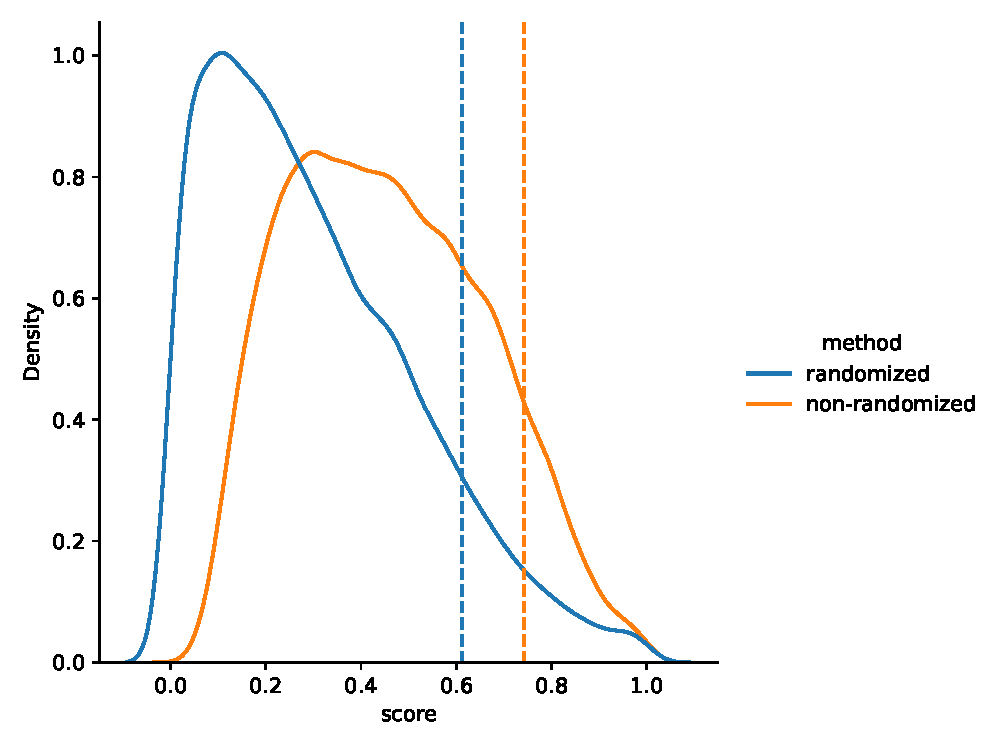
\includegraphics[width=\linewidth]{graphConformal/figures/aps_dist}
    \end{subfigure}
    \begin{subfigure}{0.48\linewidth}
        \centering
        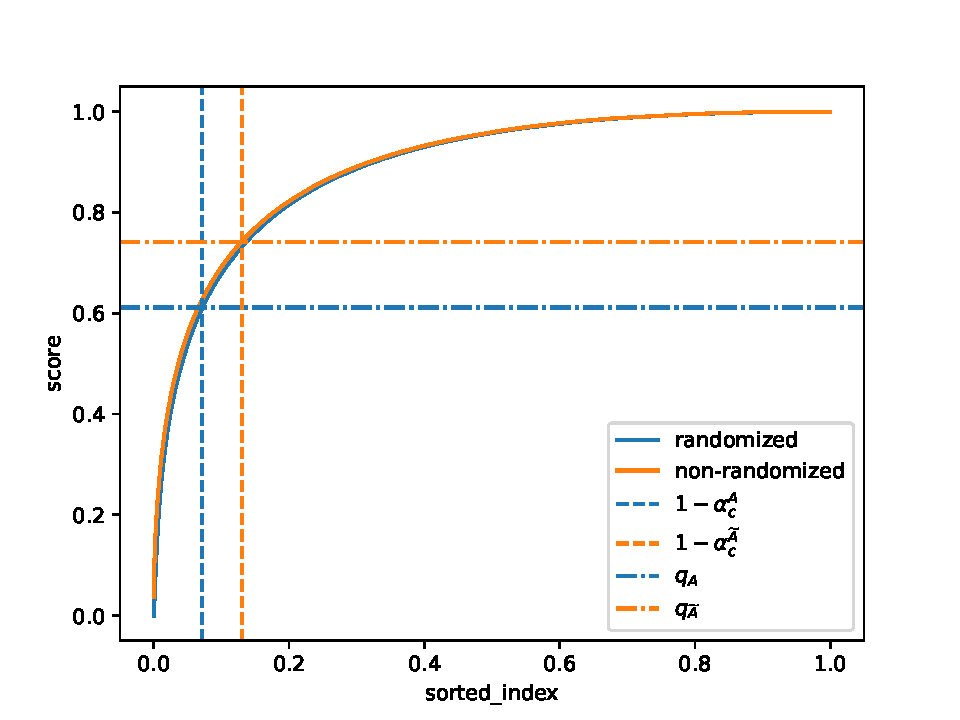
\includegraphics[width=\linewidth]{graphConformal/figures/aps_sorted}
    \end{subfigure}
    \caption{Figure showing the scores for an example dataset. (Left) shows the shift in the quantile for $A$ and $\Tilde{A}$ for the correct class. (Right) shows the shift $\alpha_c$ for $A$ and $\Tilde{A}$ using scores $A'$ for the incorrect classes.}
    \label{fig:APS:efficiency}
\end{figure}

%\pmcomment{empirical quantiles with epsilon}

%\begin{align*}
%   |S(\vx_{n+1}, u; \hat{\pi}, \tau_A)| - |\Tilda{S}(\vx_{n+1}; \hat{\pi}, \tau_{})|
%\end{align*}